\documentclass[aspectratio=169,11pt,hyperref={colorlinks=true}]{beamer}
\usetheme{boxes}
\setbeamertemplate{navigation symbols}{}
\definecolor{ibm}{RGB}{70,107,176}
\setbeamercolor{titlelike}{fg=ibm}
\setbeamercolor{structure}{fg=ibm}
\hypersetup{colorlinks,urlcolor=ibm}
\setbeamertemplate{footline}[frame number]
% Inserting graphics
\usepackage{graphicx}
% Side-by-side figures, etc
\usepackage{subfigure}
% Code snippits
\usepackage{listings}
% Color stuff
\usepackage{color}
\usepackage{amsmath}
\usepackage{tikz}
\usepackage{tipa}
\newcommand\RBox[1]{%
  \tikz\node[draw,rounded corners,align=center,] {#1};%
}
\newcommand{\light}[1]{\textcolor{gray}{#1}}
\usepackage{hyperref}
%\usecolortheme{buzz}
%\usecolortheme{wolverine}
%\usetheme{Boadilla}
\usepackage[T1]{fontenc}
\usepackage{animate}
\usepackage{pgfplotstable}
\usepackage{colortbl}
\usepackage{booktabs}

\definecolor{mygreen}{rgb}{0,0.6,0}
\definecolor{mygray}{rgb}{0.5,0.5,0.5}
\definecolor{mymauve}{rgb}{0.58,0,0.82}

\pgfplotstableset{col sep=comma, header=has colnames}

\lstset{ %
  backgroundcolor=\color{white},   % choose the background color; you must add \usepackage{color} or \usepackage{xcolor}
  breakatwhitespace=false,         % sets if automatic breaks should only happen at whitespace
  breaklines=true,                 % sets automatic line breaking
  captionpos=b,                    % sets the caption-position to bottom
  commentstyle=\color{ibm},        % comment style
  extendedchars=true,              % lets you use non-ASCII characters; for 8-bits encodings only, does not work with UTF-8
  keepspaces=true,                 % keeps spaces in text, useful for keeping indentation of code (possibly needs columns=flexible)
  keywordstyle=\color{blue},       % keyword style
  otherkeywords={*,...},           % if you want to add more keywords to the set
  numbersep=5pt,                   % how far the line-numbers are from the code
  numberstyle=\tiny\color{mygray}, % the style that is used for the line-numbers
  rulecolor=\color{black},         % if not set, the frame-color may be changed on line-breaks within not-black text (e.g. comments (green here))
  showspaces=false,                % show spaces everywhere adding particular underscores; it overrides 'showstringspaces'
  showstringspaces=false,          % underline spaces within strings only
  showtabs=false,                  % show tabs within strings adding particular underscores
  stringstyle=\color{ibm},         % string literal style
}

\setbeamerfont{caption}{series=\normalfont,size=\fontsize{8}{10}}
\setbeamertemplate{caption}{\raggedright\insertcaption\par}

\setlength{\abovecaptionskip}{0pt}
\setlength{\floatsep}{0pt}

\author[Kyra Matt Andrea]{%
    \texorpdfstring{
        \begin{columns}
            \column{.45\linewidth}
            \centering
            Kyra Wulffert\\
            \href{mailto:kwulffert@yahoo.com}{kwulffert@yahoo.com}\\
        \end{columns}
   }
   {Kyra Wulffert}
   \and
   \texorpdfstring{
       \begin{columns}
           \column{.45\linewidth}
           \centering
           Matthew Treinish\\
           \href{mailto:mtreinish@kortar.org}{mtreinish@kortar.org}\\
       \end{columns}
  }
  {Kyra Wulffert}
   \and
   \texorpdfstring{
       \begin{columns}
           \column{.45\linewidth}
           \centering
           Andrea Frittoli\\
           \href{mailto:andrea.frittoli@gmail.com}{andrea.frittoli@gmail.com}\\
       \end{columns}
  }
  {Andrea Frittoli}
}

\date{August 29, 2018}

\title[Machine Learning for CI
\hspace{2em}\insertframenumber/\inserttotalframenumber]{Machine Learning for CI}

\begin{document}

{
\setbeamertemplate{background canvas}{
\includegraphics[width=\paperwidth,height=\paperheight]{background_title.png}}
\setbeamertemplate{footline}{}
\begin{frame}[noframenumbering]
    \setbeamercolor{titlelike}{fg=white}
    \setbeamercolor{structure}{fg=white}
    \setbeamercolor{normal text}{fg=white}
    \hypersetup{colorlinks,urlcolor=white}
    \setbeamercolor{author}{fg=white}
    \setbeamercolor{date}{fg=white}
    \setbeamercolor{background}{bg=openstack}
    \titlepage{}
    \centering
    \href{https://github.com/afrittoli/ciml\_talk}{https://github.com/afrittoli/ciml\_talk}
\end{frame}
}

\section{Context}
\begin{frame}
  \frametitle{CI at Scale}
  \begin{columns}
    \column{0.6\linewidth}
      \begin{figure}
      \begin{center}
        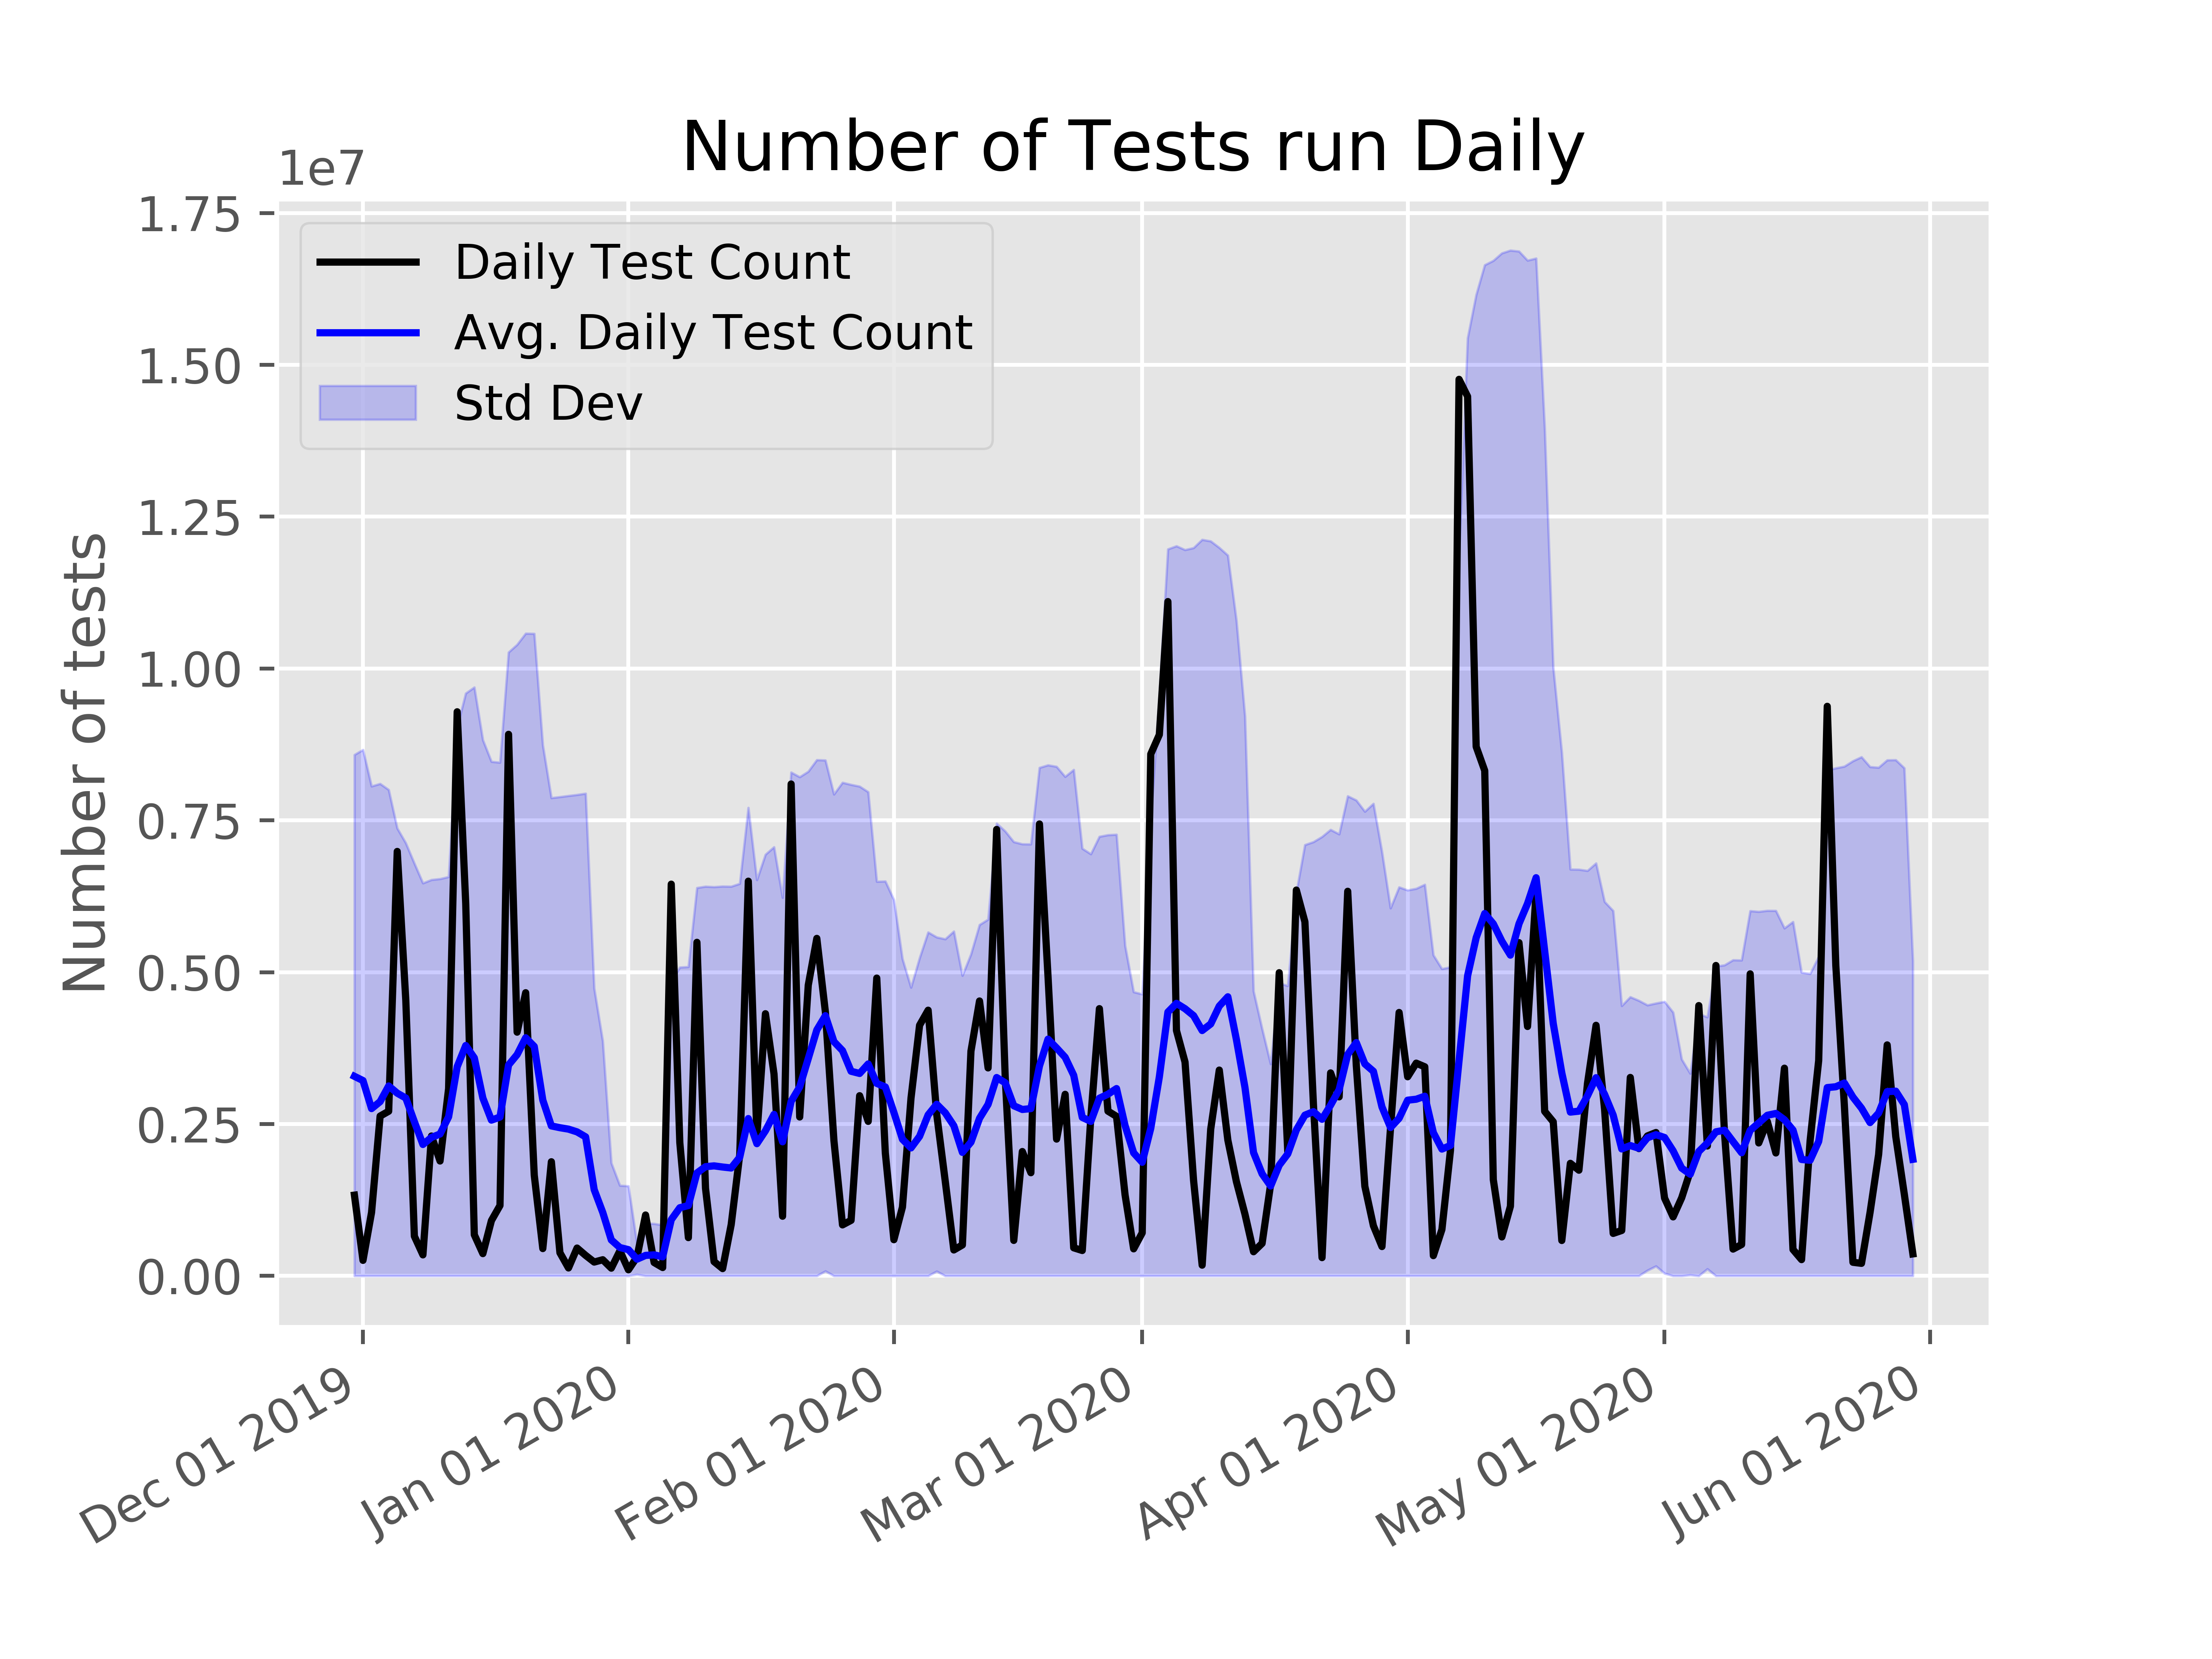
\includegraphics[width=1\textwidth]{graphs/daily_count.png}
           \caption{Source: subunit2sql-graph dailycount}
      \end{center}
      \end{figure}
    \column{0.4\linewidth}
      \begin{itemize}
          \item{Continuous Integration}
          \item{Continuous Log Data}
          \item{Lots of data, little time}
          \item{Triaging failures?}
          \item{AI to the rescue!}
      \end{itemize}
    % Add a picture, perhaps test daily count?
  \end{columns}
\end{frame}

\begin{frame}
    \frametitle{The OpenStack use case}
    \begin{columns}
      \column{0.5\linewidth}
        \begin{itemize}
            \item{Integration testing in a VM}
            \item{System logs, application logs}
            \item{Dstat data}
            \item{Gate testing}
            \item{Not only OpenStack}
        \end{itemize}
      % Add a picture with dstat graph samples
      \column{0.5\linewidth}
        \begin{figure}
        \begin{center}
          \animategraphics[autoplay,width=0.8\linewidth]{1}{graphs/100norm/1min_normalized_}{0}{99}
            \caption{Normalized system average load for different examples}
        \end{center}
        \end{figure}
    \end{columns}
\end{frame}

\section{Infrastructure}
\begin{frame}
    \frametitle{Collecting data}
    \begin{columns}
      \column{0.5\linewidth}
        \begin{figure}
        \begin{center}
          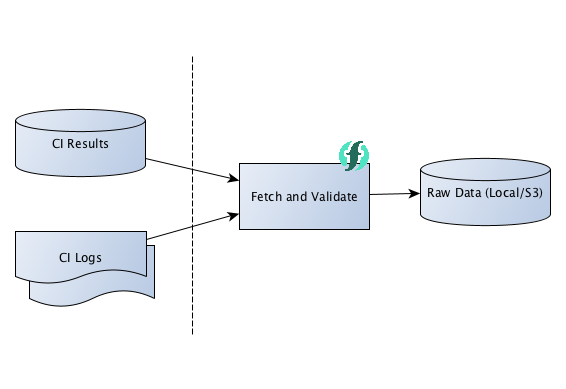
\includegraphics[width=1\textwidth]{diagrams/cache-data.png}
             \caption{Data caching diagram}
        \end{center}
        \end{figure}
      \column{0.5\linewidth}
        \begin{itemize}
            \item{Automation and repeatability}
            \item{Light-weight data validation}
            \item{Object storage for data}
            \item{Periodic Action on OpenWhisk}
        \end{itemize}
    \end{columns}
\end{frame}

\begin{frame}
    \frametitle{Experiment Workflow}
    \begin{columns}
      \column{0.4\linewidth}
        \begin{itemize}
            \item{\textbf{Visualize data}}
            \item{\textbf{Define a dataset}}
            \item{Define an experiment}
            \item{Run the training}
            \item{Collect results}
            \item{Visualize data}
        \end{itemize}
        \column{0.6\linewidth}
          \begin{figure}
            \lstinputlisting[basicstyle=\tiny,language=bash]{code/define_dataset.sh}
          \end{figure}
          \begin{figure}
            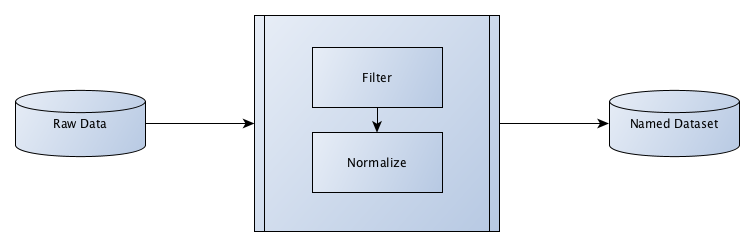
\includegraphics[width=1\textwidth]{diagrams/build-dataset.png}
            \caption{Dataset preparation diagram}
          \end{figure}
    \end{columns}
\end{frame}

\begin{frame}
    \frametitle{Experiment Workflow}
    \begin{columns}
      \column{0.4\linewidth}
        \begin{itemize}
            \item{Visualize data}
            \item{Define a dataset}
            \item{\textbf{Define an experiment}}
            \item{\textbf{Run the training}}
            \item{\textbf{Collect results}}
            \item{Visualize data}
        \end{itemize}
        \column{0.6\linewidth}
          \begin{figure}
            \lstinputlisting[basicstyle=\tiny,language=bash]{code/define_experiment.sh}
          \end{figure}
          \begin{figure}
            \lstinputlisting[basicstyle=\tiny,language=bash]{code/run_training.sh}
          \end{figure}
    \end{columns}
\end{frame}

\begin{frame}
    \frametitle{Training Infrastructure}
    \begin{columns}
      \column{0.5\linewidth}
        \begin{figure}
        \begin{center}
          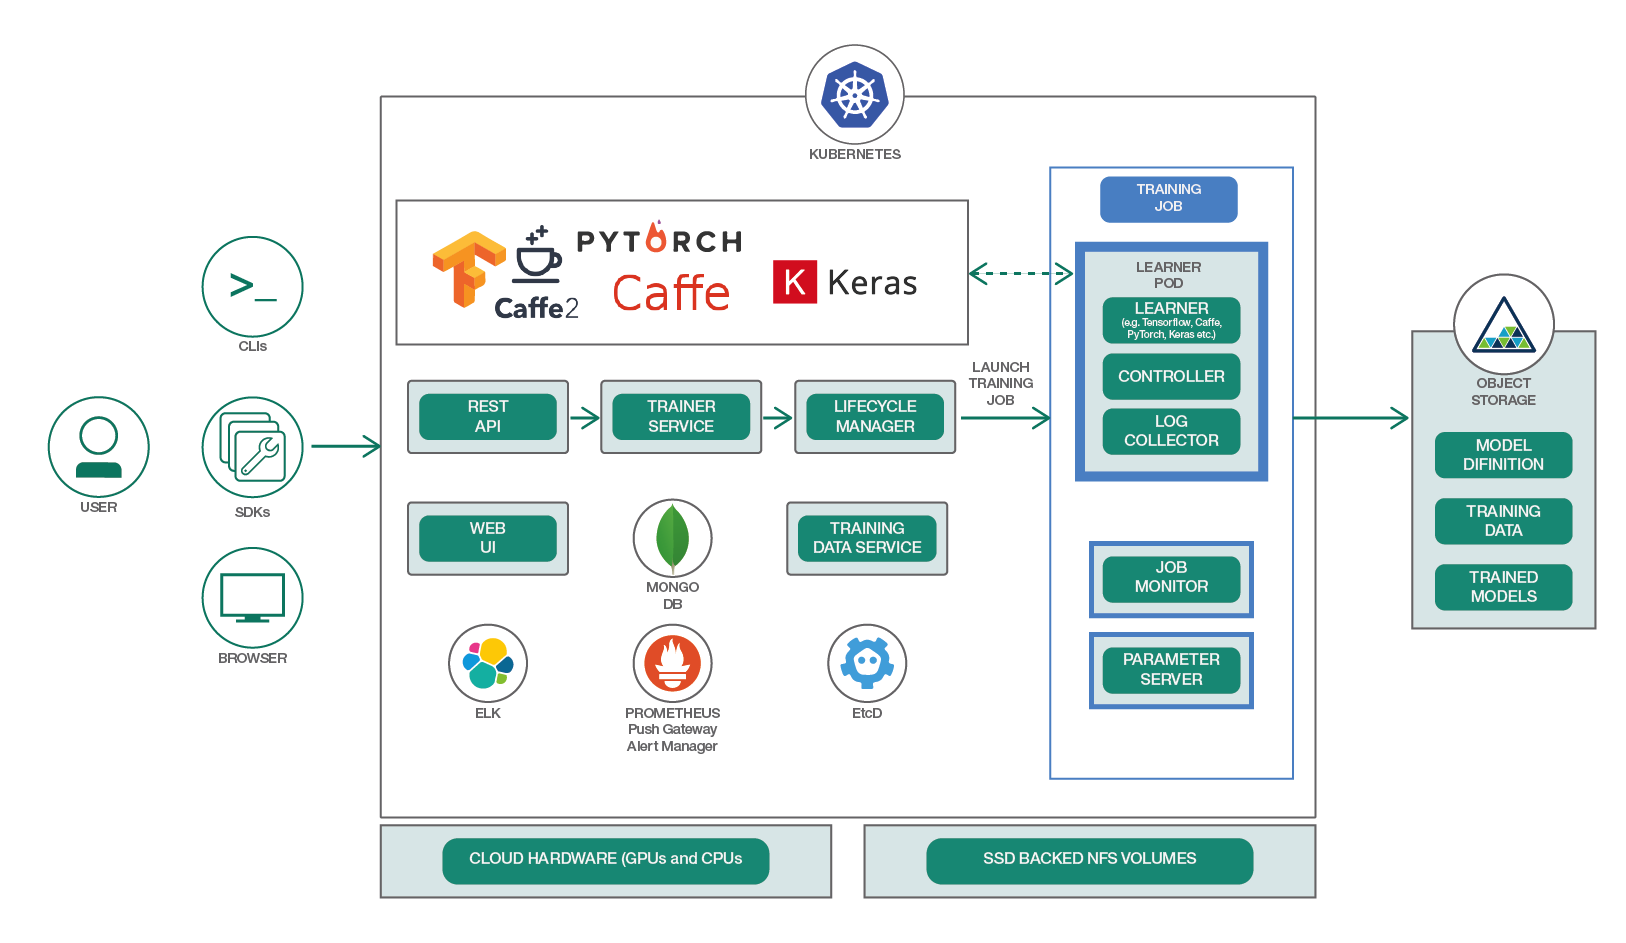
\includegraphics[width=1\textwidth]{diagrams/FfDL-Diagram.png}
             \caption{FfDL Architecture - Source: \href{https://developer.ibm.com/code/2018/03/20/democratize-ai-with-fabric-for-deep-learning/l}{https://developer.ibm.com/code/}}
        \end{center}
        \end{figure}
      \column{0.5\linewidth}
        \begin{itemize}
          \item{TensorFlow Estimator API}
          \item{CIML wrapper}
          \item{ML framework interchangable}
          \item{Training Options:}
          \begin{itemize}
            \item{Run on a local machine}
            \item{Helm deploy CIML, run in containers}
            \item{\light{Submit training jobs to Ffdl}}
            \item{\light{Kubeflow}}
          \end{itemize}
        \end{itemize}
    \end{columns}
\end{frame}

\begin{frame}
    \frametitle{Prediction}
    \begin{columns}
      \column{0.5\linewidth}
        \begin{itemize}
            \item{Event driven: near real time}
            \item{No request to serve the prediction to}
            \item{MQTT Trigger from the CI system}
            \item{CIML produces the prediction}
            \item{Trusted Source: Continuous Training}
        \end{itemize}
      \column{0.5\linewidth}
        \begin{itemize}
          \item{CIML kubernetes app components:}
          \begin{itemize}
            \item{MQTT Client receives events}
            \item{Data module fetches and prepares data}
            \item{TensorFlow wrapper issues the prediction}
            \item{Example: comment back on Gerrit/Github}
          \end{itemize}
        \end{itemize}
    \end{columns}
\end{frame}

\section{Data}
\begin{frame}
    \frametitle{Data Selection}
    \begin{columns}
      \column{0.5\linewidth}
        \begin{itemize}
            \item{What is dstat data}
            \item{Experiment reproducibility}
            \item{Dataset selection}
            \begin{itemize}
              \item{Dstat feature selection}
              \item{Data resolution (down-sampling)}
            \end{itemize}
        \end{itemize}
      \column{0.5\linewidth}
      \begin{table}[h!]
        \begin{center}
          \caption{Sample of dstat data}
          \label{dstat_sample}
          \resizebox{0.7\linewidth}{!}{
            \pgfplotstabletypeset[
              columns/time/.style={string type},
              every head row/.style={after row=\midrule},
              every first row/.style={before row=\rowcolor{mygray}},
              every nth row={5}{before row=\rowcolor{mygray}},
              columns/usr/.style={column type/.add={>{\columncolor[gray]{.8}}}{}},
              columns/1m/.style={column type/.add={>{\columncolor[gray]{.8}}}{}},
            ]{code/dstat_sample.csv}
          }
        \end{center}
     \end{table}
  \end{columns}
\end{frame}

\begin{frame}
    \frametitle{Data Normalization}
    \begin{columns}
      \column{0.5\linewidth}
        \begin{itemize}
            \item{Unrolling}
            % (formula) x - mean / xmax - mmin
        \end{itemize}
        \begin{table}[h!]
          \begin{center}
            \caption{Sample of unrolled data}
            \label{unrolled_sample}
            \resizebox{0.6\linewidth}{!}{
              \pgfplotstabletypeset[
                every head row/.style={after row=\midrule},
              ]{code/unrolled_sample.csv}
            }
          \end{center}
       \end{table}
      \column{0.5\linewidth}
      \begin{itemize}
          \item{Normalizing}
          % (formula) x - mean / xmax - xmin
      \end{itemize}
      \begin{table}[h!]
        \begin{center}
          \caption{Sample of normalized data}
          \label{normalized_sample}
          \resizebox{0.6\linewidth}{!}{
            \pgfplotstabletypeset[
              every head row/.style={after row=\midrule},
            ]{code/normalized_sample.csv}
          }
        \end{center}
     \end{table}
     \end{columns}
\end{frame}

\begin{frame}
    \frametitle{Building the dataset}
    \begin{columns}
      \column{0.5\linewidth}
        \begin{figure}
        \begin{center}
          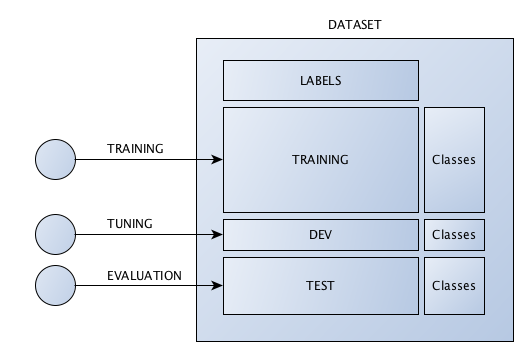
\includegraphics[width=0.9\textwidth]{diagrams/dataset.png}
             \caption{Structure of a dataset}
        \end{center}
        \end{figure}
      \column{0.5\linewidth}
        \begin{itemize}
            \item{Split in training, dev, test}
            \item{Obtain classes}
            \item{Store normalized data on s3}
            \item{Input function for training}
            \item{Input function for evaluation}
        \end{itemize}
    \end{columns}
\end{frame}

\section{Experiments}
\begin{frame}
    \frametitle{DNN - Binary Classification}
    \begin{columns}
      \column{0.5\linewidth}
        \begin{itemize}
            \item{Classes: Passed or Failed}
            \item{Supervised training}
            \item{TensorFlow \emph{DNNClassifier}, classes=2}
            \item{Dataset:}
            \begin{itemize}
              \item{CI Job "tempest-full"}
              \item{Gate pipeline only}
              \item{2000 examples, 1400 training, 600 test}
            \end{itemize}
            \item{Hyper-parameters:}
            \begin{itemize}
              \item{Activation function: ReLU}
              \item{Output layer: Sigmoid}
              \item{Optimizer: Adagrad}
              \item{Learning rate (initial): 0.05}
              \item{5 hidden layers, 100 units per layer}
              \item{Batch Size: 128, Epochs: 500}
            \end{itemize}
        \end{itemize}
      \column{0.5\linewidth}
        \begin{figure}
        \begin{center}
          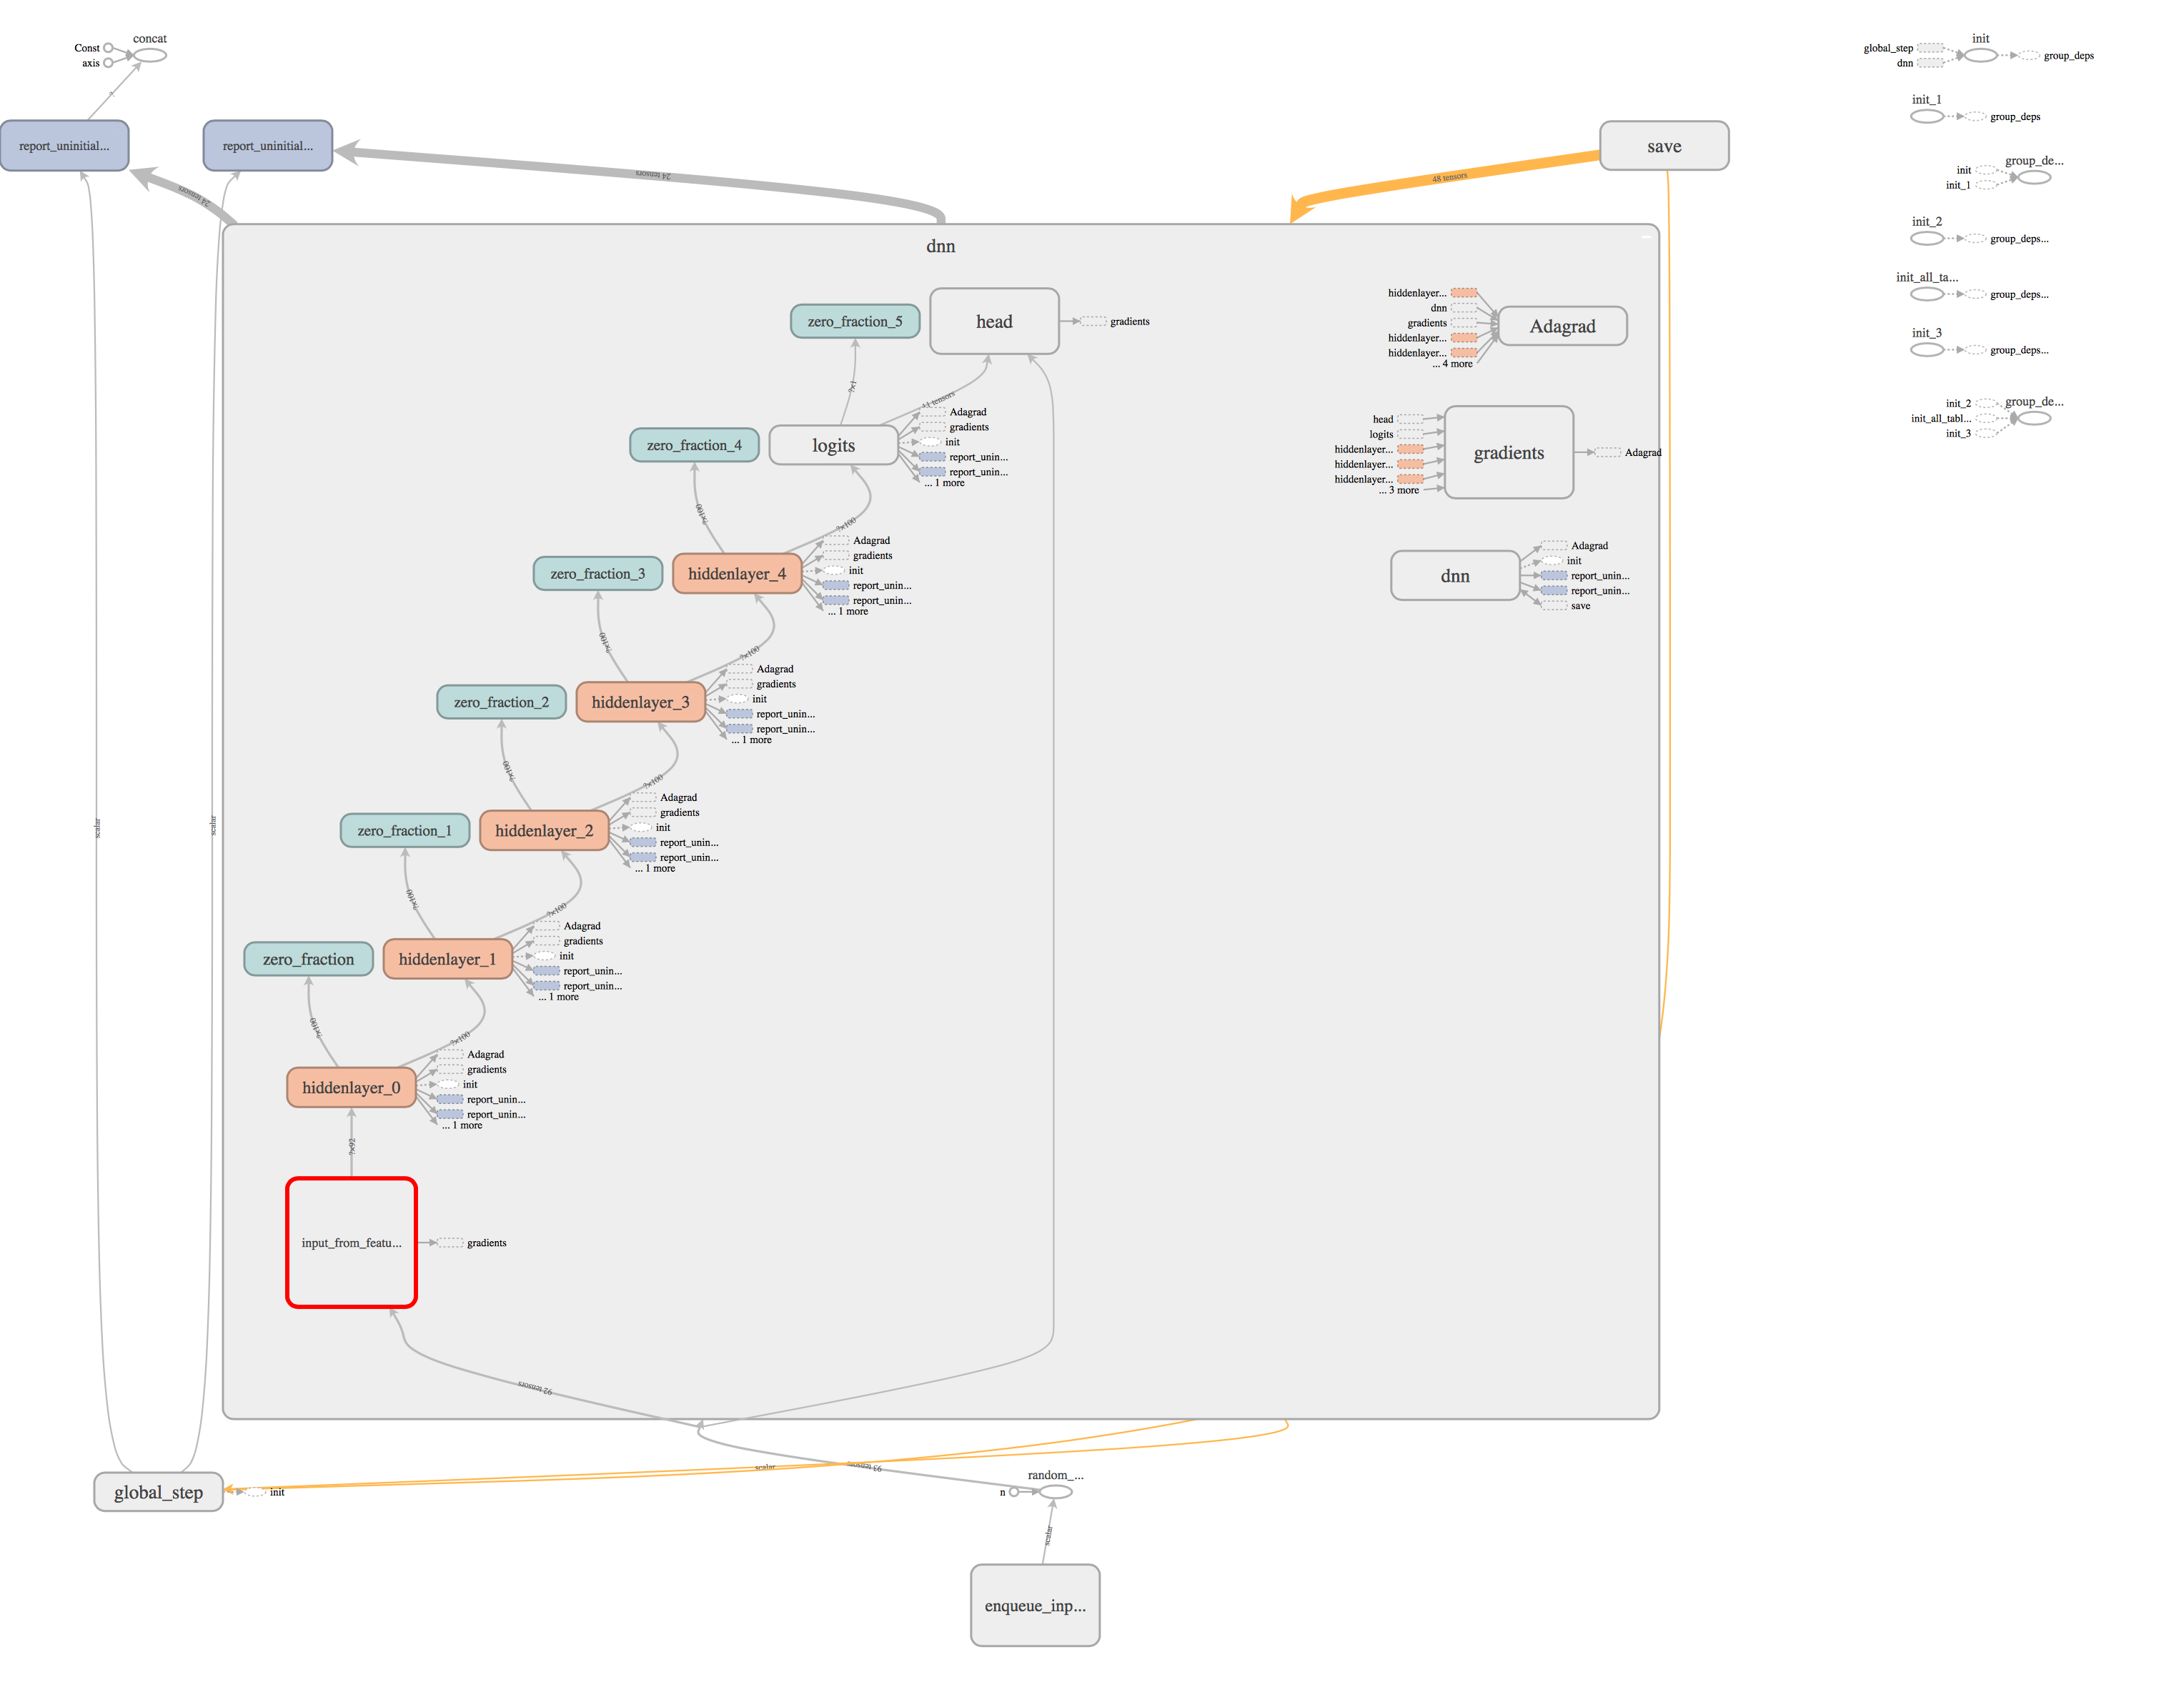
\includegraphics[width=0.9\textwidth]{diagrams/binary_class_network_diagram.png}
             \caption{Network Graph - Source: TensorBoard}
        \end{center}
        \end{figure}
    \end{columns}
\end{frame}

\begin{frame}
    \frametitle{DNN - Binary Classification}
    \begin{columns}
      \column{0.5\linewidth}
        \begin{itemize}
            \item{Selecting the best feature set}
            \item{Primary metric: accuracy}
            \item{Aim for lower loss, caveat: overfitting}
            \item{Key:}
            \begin{itemize}
              \item{\textbf{usr}: User CPU}
              \item{\textbf{used}: Used Memory}
              \item{\textbf{1m}: System Load - 1min Average}
              \item{Data Resolution: \textbf{1min}}
              \item{Source: TensorFlow evaluation output}
            \end{itemize}
            \item{Winner: (\textbf{usr}, \textbf{1m}) tuple}
            \item{Accuracy achieved: \emph{\textbf{0.995}}}
            \item{3 mistakes on a 600 test set}
        \end{itemize}
      \column{0.5\linewidth}
        \begin{center}
        \begin{figure}
          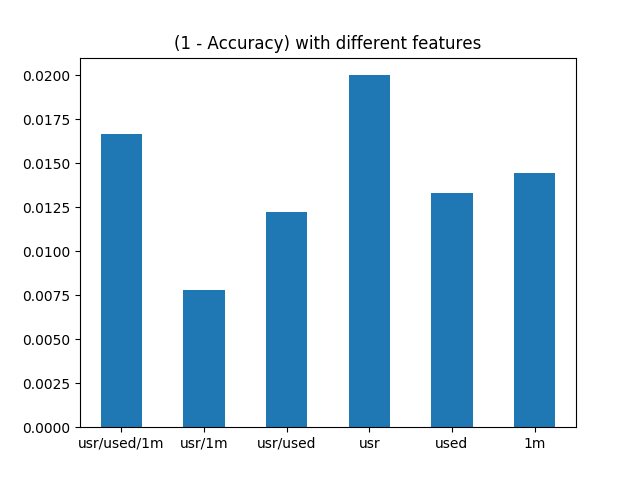
\includegraphics[width=0.8\textwidth,height=0.4\textheight]{graphs/accuracy_by_feature-status.png}
        \end{figure}
        \begin{figure}
          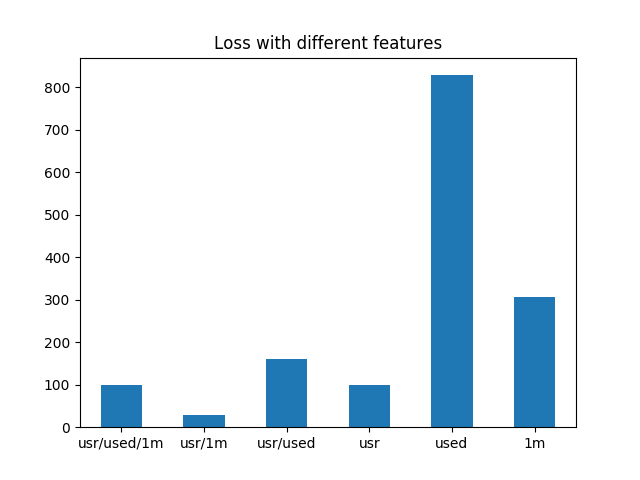
\includegraphics[width=0.8\textwidth,height=0.4\textheight]{graphs/loss_by_feature-status.png}
        \end{figure}
      \end{center}
  \end{columns}
\end{frame}

\begin{frame}
    \frametitle{DNN - Binary Classification}
    \begin{columns}
      \column{0.5\linewidth}
        \begin{itemize}
            \item{Selecting the data resolution}
            \item{Primary metric: accuracy}
            \item{Aim for lower loss, caveat: overfitting}
            \item{Note: careful with NaN after down-sampling}
            \item{Key:}
            \begin{itemize}
              \item{Original data frequency: 1s}
              \item{x-axis: new sampling rate}
              \item{Source: TensorFlow evaluation output}
              \item{Features: (\textbf{usr}, \textbf{1m})}
            \end{itemize}
            \item{Winner: \textbf{1min}}
            \item{Accuracy achieved: \emph{\textbf{0.995}}}
            \item{3 mistakes on a 600 test set}
        \end{itemize}
      \column{0.5\linewidth}
        \begin{center}
        \begin{figure}
          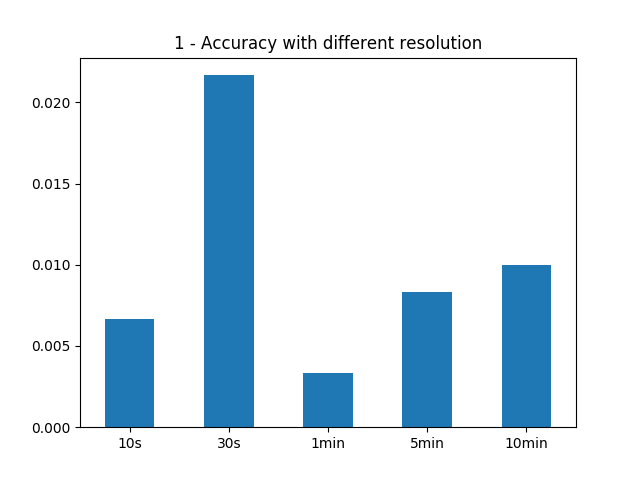
\includegraphics[width=0.8\textwidth,height=0.4\textheight]{graphs/accuracy_by_sampling-status.png}
        \end{figure}
        \begin{figure}
          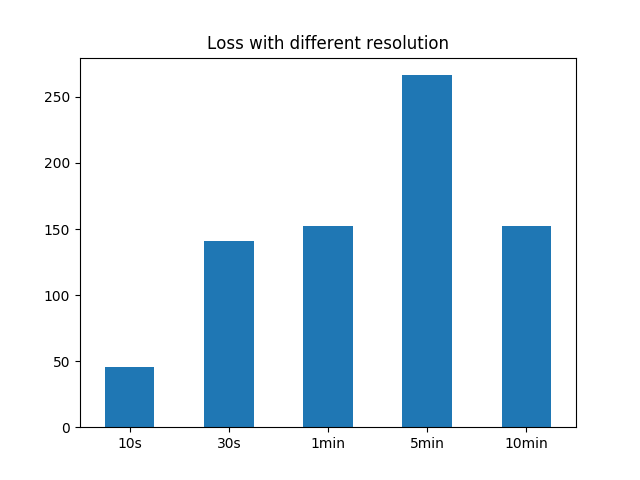
\includegraphics[width=0.8\textwidth,height=0.4\textheight]{graphs/loss_by_sampling-status.png}
        \end{figure}
      \end{center}
  \end{columns}
\end{frame}

\begin{frame}
    \frametitle{Changing test job}
    \begin{columns}
      \column{0.5\linewidth}
        \begin{table}[h!]
          \begin{center}
            \label{binary_eval_compare}
            \resizebox{1\linewidth}{!}{
              \pgfplotstabletypeset[
                precision=3,
                columns/metric/.style={string type},
                every head row/.style={after row=\midrule},
                every even row={5}{before row=\rowcolor{mygray}},
              ]{code/usr_1m-1min-status-eval-compare.csv}
            }
          \end{center}
       \end{table}
      \column{0.5\linewidth}
        \begin{itemize}
            \item{Train with "tempest-full"}
            \item{Evaluating with "tempest-full-py3"}
            \begin{itemize}
              \item{Similar setup, uses python3}
              \item{It does not include swift and swift tests}
              \item{600 examples evaluation set}
            \end{itemize}
            \item{Dataset and training setup:}
            \begin{itemize}
              \item{Features: (usr, 1m)}
              \item{Resolution: 1min}
              \item{Same hyper-parameters}
            \end{itemize}
        \end{itemize}
    \end{columns}
\end{frame}

\begin{frame}
    \frametitle{Binary Classification - Summary}
    \begin{columns}
      \column{0.4\linewidth}
        \begin{itemize}
            \item{User CPU and 1min Load Avg}
            \item{Resolution: 1 minute is enough}
            \item{High accuracy: \emph{\textbf{0.995}}}
            \item{High auc\_precision\_recall: \emph{\textbf{0.945}}}
        \end{itemize}
      \column{0.6\linewidth}
        \begin{figure}
          \begin{center}
            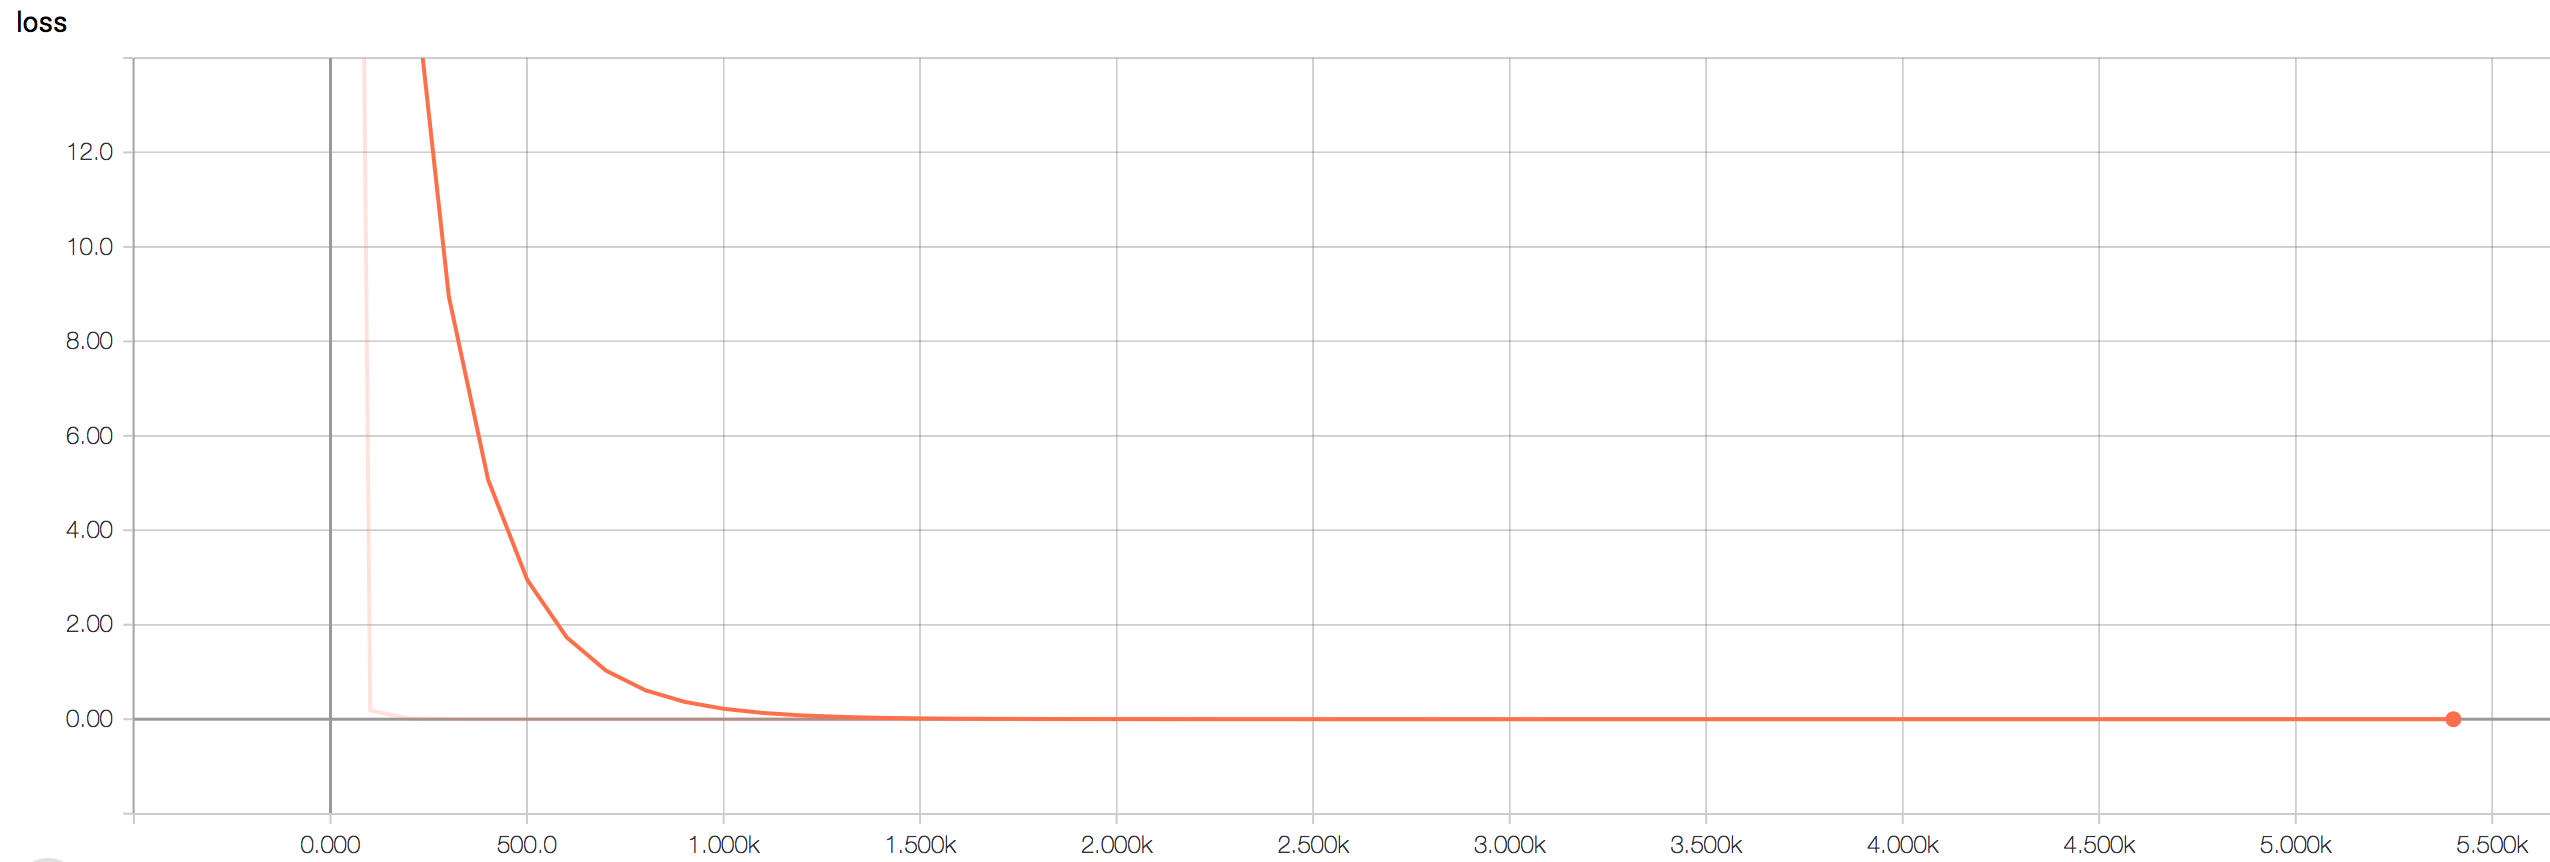
\includegraphics[width=0.9\textwidth,height=0.5\textheight]{graphs/cpu_1m-1min-status_loss_curve.png}
              \caption{Training Loss - usr/1m, 1min - Source: TensorBoard}
          \end{center}
        \end{figure}
      \end{columns}
\end{frame}

\begin{frame}
    \frametitle{DNN - Multi Class}
    \begin{columns}
      \column{0.5\linewidth}
        \begin{itemize}
            \item{Classes: Hosting Cloud Provider}
            \item{Supervised training}
            \item{TensorFlow \emph{DNNClassifier}, classes=\textbf{9}}
            \item{Dataset:}
            \begin{itemize}
              \item{CI Job "tempest-full"}
              \item{Gate pipeline only}
              \item{2000 examples, 1400 training, 600 test}
            \end{itemize}
            \item{Hyper-parameters:}
            \begin{itemize}
              \item{Activation function: ReLU}
              \item{Output layer: Sigmoid}
              \item{Optimizer: Adagrad}
              \item{Learning rate (initial): 0.05}
              \item{5 hidden layers, 100 units per layer}
              \item{Batch Size: 128, Epochs: 500}
            \end{itemize}
        \end{itemize}
      \column{0.5\linewidth}
        \begin{figure}
        \begin{center}
          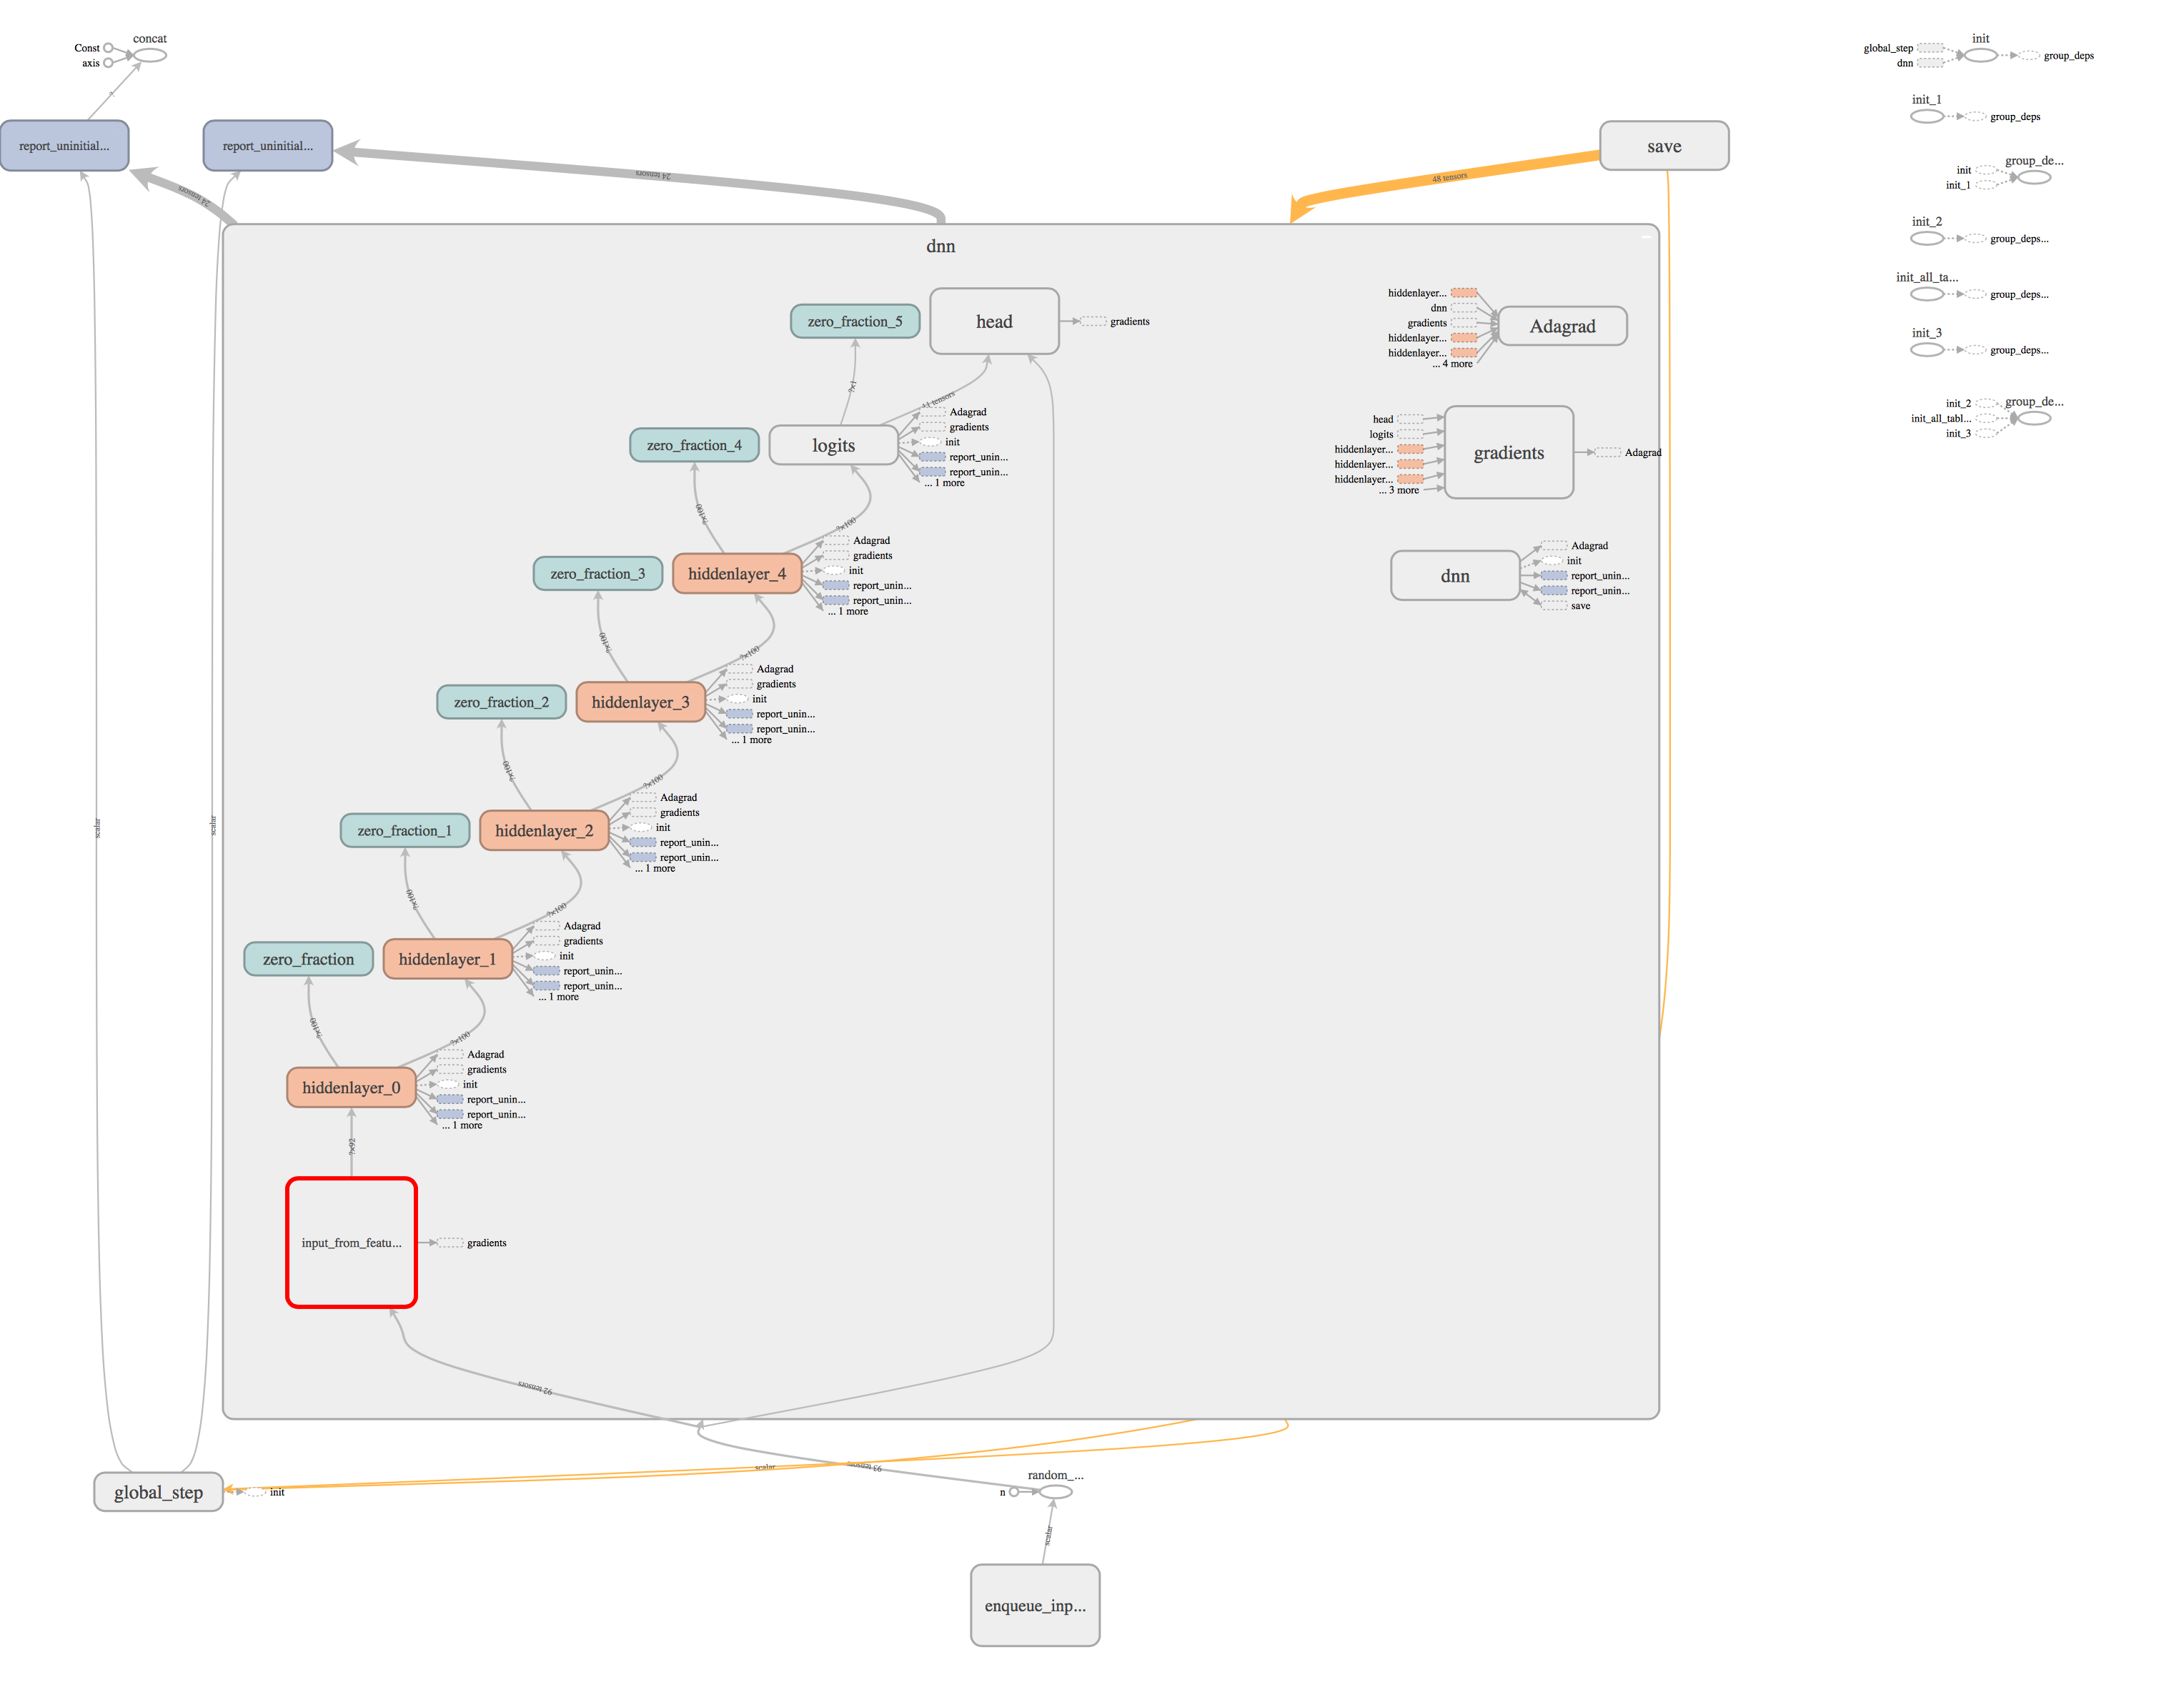
\includegraphics[width=0.9\textwidth]{diagrams/binary_class_network_diagram.png}
             \caption{Network Graph - Source: TensorBoard}
        \end{center}
        \end{figure}
    \end{columns}
\end{frame}

\begin{frame}
    \frametitle{DNN - Multi Class}
    \begin{center}
      \begin{itemize}
        \item{Features: (usr, 1m)}
        \item{Resolution: 1min}
        \item{Accuracy achieved: \emph{\textbf{0.995}}}
      \end{itemize}
    \end{center}
\end{frame}

\begin{frame}
    \frametitle{Multi Class - Growing back number of features}
    \begin{columns}
      \column{0.5\linewidth}
        \begin{itemize}
            \item{Selecting the best feature set}
            \item{Primary metric: accuracy}
            \item{Aim for lower loss, caveat: overfitting}
            \item{Key:}
            \begin{itemize}
              \item{\textbf{usr}: User CPU}
              \item{\textbf{used}: Used Memory}
              \item{\textbf{1m}: System Load - 1min Average}
              \item{Data Resolution: \textbf{1min}}
              \item{Source: TensorFlow evaluation output}
            \end{itemize}
            \item{Winner: (\textbf{usr}, \textbf{1m}) tuple}
            \item{Accuracy achieved: \emph{\textbf{0.995}}}
            \item{3 mistakes on a 600 test set}
        \end{itemize}
      \column{0.5\linewidth}
        \begin{center}
        \begin{figure}
          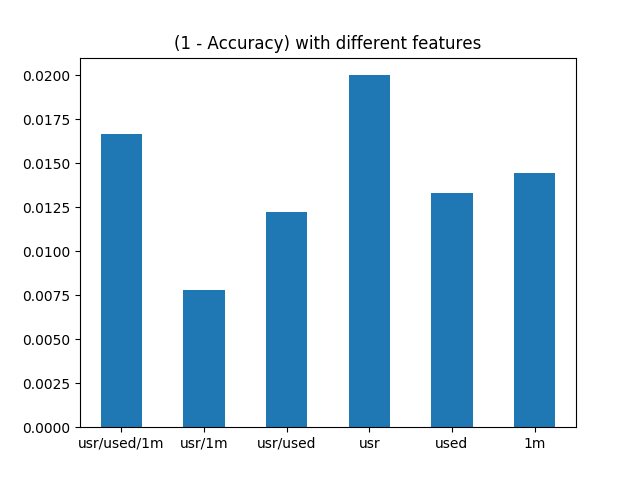
\includegraphics[width=0.8\textwidth,height=0.4\textheight]{graphs/accuracy_by_feature-status.png}
        \end{figure}
        \begin{figure}
          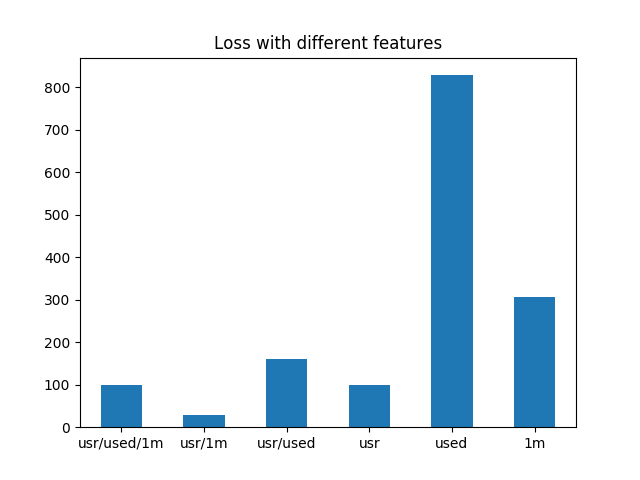
\includegraphics[width=0.8\textwidth,height=0.4\textheight]{graphs/loss_by_feature-status.png}
        \end{figure}
      \end{center}
  \end{columns}
\end{frame}

\begin{frame}
    \frametitle{Multi Class - Increasing Resolution}
    \begin{itemize}
        \item{Playing with the network topology}
    \end{itemize}
\end{frame}

\begin{frame}
    \frametitle{Multi Class - Playing with the network topology}
    \begin{itemize}
        \item{Playing with the network topology}
    \end{itemize}
\end{frame}

\begin{frame}
    \frametitle{Multi Class - Reducing the number of classes}
    \begin{itemize}
        \item{Reducing the number of classes}
        \item{What does that mean}
        \item{Why did it work}
    \end{itemize}
\end{frame}

\begin{frame}
    \frametitle{Multi Class - Changing test job}
    \begin{itemize}
        \item{Train with a CI Job}
        \item{Evaluating with another CI Job (as well)}
    \end{itemize}
\end{frame}

\begin{frame}
    \frametitle{Multi Class - Summary}
    \begin{itemize}
        \item{Topology / Hyperparameters}
        \item{Loss curve}
    \end{itemize}
\end{frame}

\section{Conclusions}
\begin{frame}
  \frametitle{Conclusions}
  \begin{itemize}
      \item{Summary on DNN binary classification}
      \item{Summary on DNN multi class}
      \item{Collect data}
      \item{Know your data}
      \item{Work with cloud tools}
  \end{itemize}
\end{frame}

\begin{frame}
  \frametitle{Future Work}
  \begin{itemize}
      \item{Complete setup of the pipeline}
      \item{Human curated dataset for supervised training}
      \item{Making our life easier}
      \item{Integrate with real life CI system}
      \item{Explore job portability}
  \end{itemize}
\end{frame}

\section{Questions}
\begin{frame}[c]
    %\frametitle{Questions?}
    \begin{center}
        \Huge Thank you!\\Questions?
    \end{center}
\end{frame}

\end{document}
